% Keep nonacm until this draft is actually submitted to ACM/TOMS.
\documentclass[manuscript,nonacm]{acmart}

\setcopyright{none}
\settopmatter{printacmref=false}
\raggedbottom{}
\acmJournal{TOMS}

\title{Validation Architecture in delaunay}

\author{Adam Getchell}
\email{adam@adamgetchell.org}
\orcid{0000-0002-0797-0021} % chktex 8
\affiliation{%
  \institution{The George Washington University}
  \city{Washington}
  \state{DC}
  \country{USA}
}

% Keep this explicit so CI rebuilds do not rewrite the reviewer-copy date.
\date{July 6, 2026}

% Authorship note:
% This source is intentionally an author-facing outline. Agents may maintain
% TeX structure, build tooling, citation plumbing, figures, and TODO prompts,
% but Adam writes the substantive paper prose.
\newcommand{\AuthorTodo}[1]{\textbf{Author TODO.} #1}
\begin{abstract}
  \AuthorTodo{Write the abstract in your own words.}
\end{abstract}

\keywords{TODO author-supplied keywords}

\begin{document}
\maketitle

\section{Introduction}

\begin{itemize}
  \item \AuthorTodo{State the problem and motivation.}
  \item \AuthorTodo{Explain why validation architecture matters for a
    scientific computational-geometry library.}
  \item \AuthorTodo{Summarize the central contribution in your own words.}
  \item \AuthorTodo{Preview the paper structure.}
\end{itemize}

Applications such as Causal Dynamical Triangulation (CDT) require a robust and
reliable triangulation library, capable of maintaining correct properties of the
triangulation in simulations that may alter their structure millions
of times per
simulation.
These invariant properties should be verifiable during construction
and mutation,
and violations of these properties should be detectable and diagnosable, so that
fixable errors may be corrected and unfixable errors may be reported.

Delaunay is a Rust library for constructing and mutating triangulations with
insertion, deletion, and bi-stellar k-flip operations, while maintaining a range
of invariant properties important for the construction of Pseudo- and
Piecewise-Linear (PL) manifolds,
the evaluation of geometric predicates, and the embedding of
triangulations in Euclidean,
toroidal, and spherical spaces.

\AuthorTodo{Qualify the preceding overview so the ordinary mutable
  Euclidean/toroidal workflows are distinguished from the separate bounded
\(S^2\)/\(S^3\) spherical prototype.}

\section{Background and Definitions}

\begin{itemize}
  \item \AuthorTodo{Define the triangulation, simplex, ridge, facet, and
    realization terms used throughout the paper.}
  \item \AuthorTodo{Introduce PL-manifold terminology and the link condition.}
  \item \AuthorTodo{Introduce Euclidean, toroidal, and spherical realization
    models.}
  \item \AuthorTodo{Introduce Delaunay and future geometric-predicate
    terminology.}
\end{itemize}

\section{Validation Hierarchy}

\begin{figure}[htbp]
  \centering
  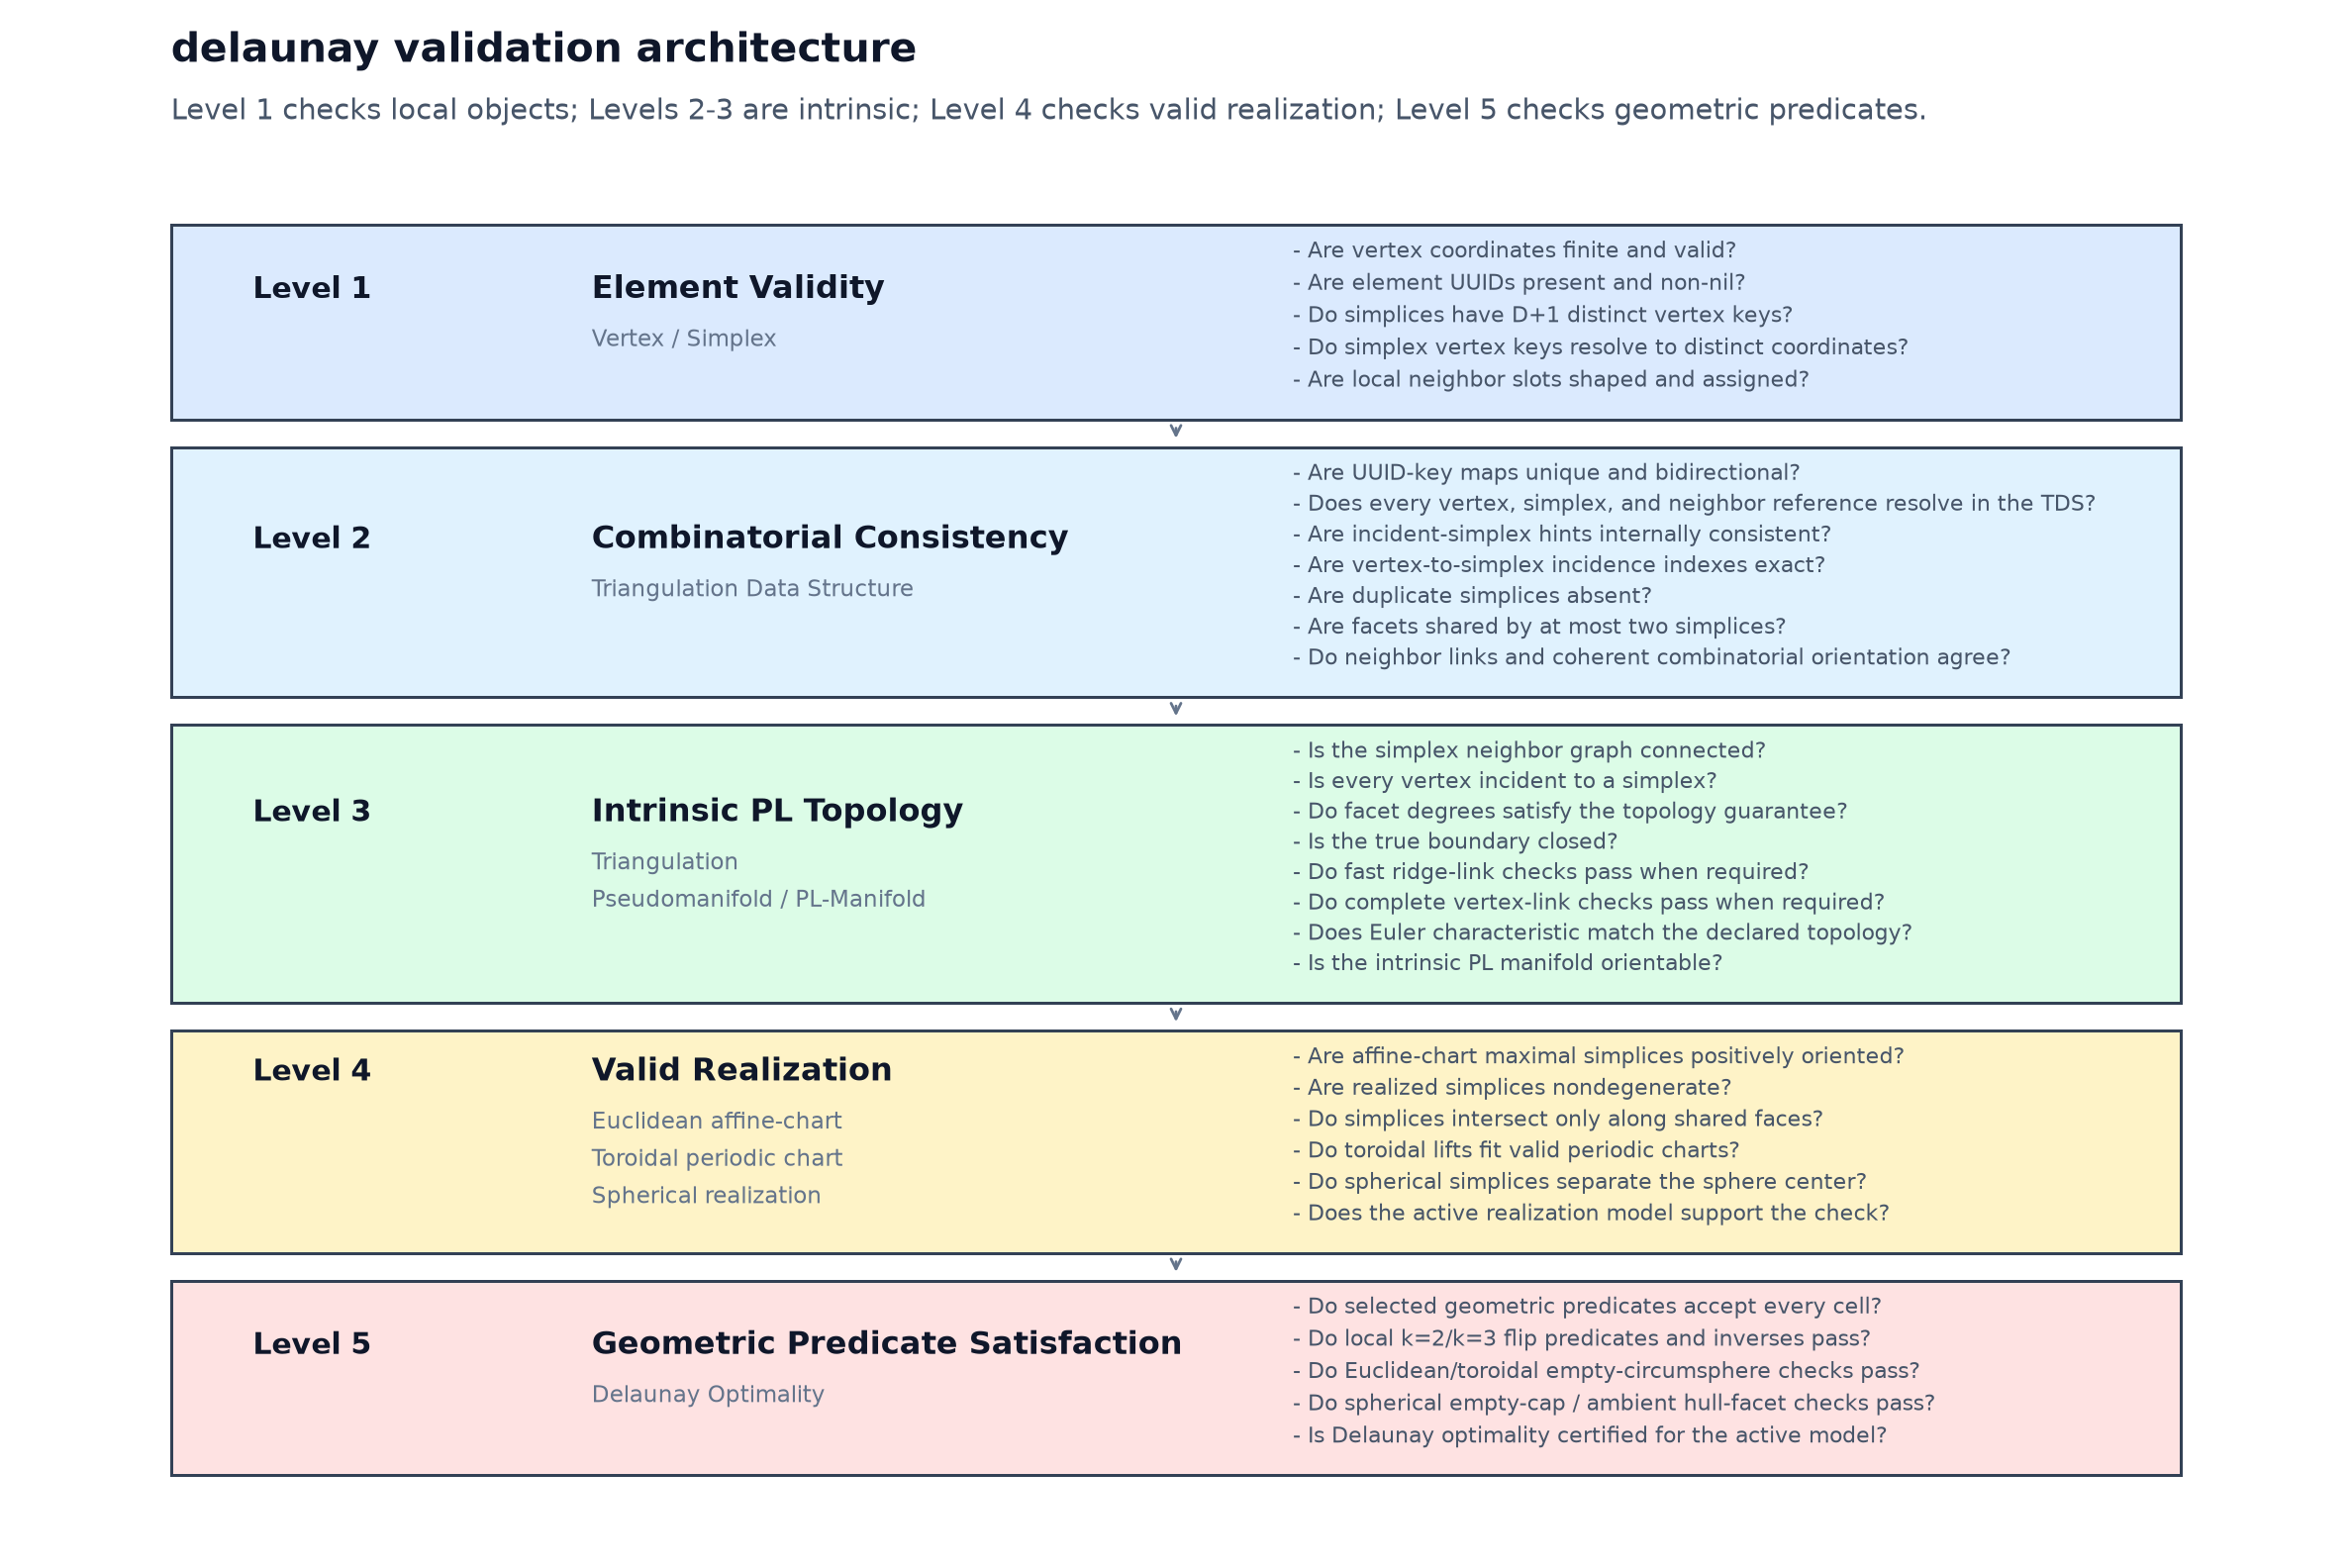
\includegraphics[width=0.95\linewidth]
  {../docs/assets/validation/validation_hierarchy.png}
  \caption{Overview of the validation hierarchy in
  delaunay}\label{fig:validation-hierarchy}
  \Description{The 5-level validation hierarchy in delaunay. Level 1:
    Element Validity; Level 2: Combinatorial Consistency; Level 3: Intrinsic
    PL Topology; Level 4: Valid Realization; Level 5: Geometric Predicate
  Satisfaction.}
\end{figure}

\subsection{Level 1: Element Validity}

\begin{itemize}
  \item \AuthorTodo{Describe what individual vertices, simplices, facets, and
    coordinates must prove locally.}
  \item \AuthorTodo{Explain what this level deliberately does not check.}
\end{itemize}

\subsection{Level 2: Combinatorial Consistency}

\begin{itemize}
  \item \AuthorTodo{Describe adjacency, incidence, neighbor symmetry, and TDS
    integrity.}
  \item \AuthorTodo{Distinguish coherent stored simplex orderings, including
    periodic quotient facets, from intrinsic orientability.}
  \item \AuthorTodo{Explain the separation from topology and geometry.}
\end{itemize}

\subsection{Level 3: Intrinsic PL Topology}

\begin{itemize}
  \item \AuthorTodo{State the PL-manifold and boundary conditions.}
  \item \AuthorTodo{Discuss pseudomanifold and strict PL-manifold policy
    choices.}
  \item \AuthorTodo{Describe the 2D/3D intrinsic orientation witness and
    periodic quotient parity constraints.}
  \item \AuthorTodo{Explain why this layer is independent of Euclidean,
    toroidal, and spherical realizations.}
\end{itemize}

\subsection{Level 4: Valid Realization}

\begin{itemize}
  \item \AuthorTodo{Use the terminology stack: Level 4 Valid Realization;
      Euclidean/toroidal valid affine-chart realization; spherical valid
      spherical realization; Level 5 Geometric Predicate Satisfaction / Delaunay
    Optimality.}
  \item \AuthorTodo{Describe valid realization in the active ambient
    model.}
  \item \AuthorTodo{Compare Euclidean/toroidal affine-chart realizations and
    spherical realizations.}
  \item \AuthorTodo{Keep positive geometric orientation distinct from Level 2
    stored coherence and Level 3 intrinsic orientability.}
  \item \AuthorTodo{Explain why realization validity is a precondition for
    geometric predicates.}
  \item \AuthorTodo{Introduce two realized \(d\)-simplices with vertices
      \(a_0,\ldots,a_d\) and \(b_0,\ldots,b_d\), vertex labels
      \(\ell_i\) and \(m_j\), and shared-label set \(S\), then explain the exact
      shared-face intersection program in
    Equation~\ref{eq:shared-face-intersection-lp}.}
    \begin{equation}
      \label{eq:shared-face-intersection-lp}
      \begin{aligned}
        z^\star
        ={}& \underset{\alpha_i,\beta_j \geq 0}{\operatorname{maximize}}
        && \sum_{\ell_i \notin S} \alpha_i
        + \sum_{m_j \notin S} \beta_j \\
        & \text{\rm subject to}
        && \sum_{i=0}^{d} \alpha_i a_i
        = \sum_{j=0}^{d} \beta_j b_j, \\
        &&& \sum_{i=0}^{d} \alpha_i = 1,
        \qquad \sum_{j=0}^{d} \beta_j = 1 .
      \end{aligned}
    \end{equation}
  \item \AuthorTodo{Explain the three exact outcomes: infeasibility proves the
      simplices disjoint; \(z^\star=0\) proves every feasible intersection point
      is confined to the shared face; and \(z^\star>0\) supplies barycentric
    weight on non-shared labels for a typed intersection witness.}
  \item \AuthorTodo{Explain how revised-simplex basis navigation replaces
      exhaustive active-set enumeration of the intersection polytope on the
      common path and removes the bottleneck exposed by the 4D and 5D Level 4
    checks.}
  \item \AuthorTodo{Describe the filtered-exact hierarchy: bounding-box,
      separating-facet, orientation, and shared-face normal tests reject or
      certify easy pairs; floating-point simplex phases propose axes and bases;
      proved floating-point error bounds or exact rational primal/dual checks
      certify accepted results; and active-set enumeration remains the
    conservative fallback.}
  \item \AuthorTodo{Describe how exact finite-\texttt{f64} systems use the
      runtime-dispatched fraction-free Bareiss solver from \texttt{la-stack},
    while general rational systems retain the \texttt{BigRational} fallback.}
  \item \AuthorTodo{Treat the broader independent randomized and degenerate
      2D--5D agreement campaign and representative before/after benchmarks as
    v0.8.1 work tracked by issue \#482.}
  \item \AuthorTodo{Do not present the bounded v0.8.0 4D and 5D slow-test probes
      as performance evidence. Coordinate any Level 5 all-violations performance
    claims with the separate v0.8.1 work in issue \#483.}
\end{itemize}

\subsection{Level 5: Geometric Predicates}

\begin{itemize}
  \item \AuthorTodo{Describe Delaunay as the first implemented predicate
    family.}
  \item \AuthorTodo{Explain how Euclidean, toroidal, and spherical Delaunay
    predicates differ.}
  \item \AuthorTodo{Leave room for regular, weighted, constrained, Gabriel,
    alpha, and future predicate families.}
\end{itemize}

\section{Implementation Architecture}

\begin{center}
  \begin{minipage}{\textwidth}
    \captionof{table}{Public validation API by owning layer.}
    \label{tab:validation-api}
    \small
    \begin{tabular}{@{}cp{0.88\textwidth}@{}}
      \toprule
      Level & Canonical public surface \\
      \midrule
      1 & \texttt{Vertex::is\_valid} / \texttt{vertex\_report};
      \texttt{Simplex::is\_valid} / \texttt{simplex\_report} \\
      2 & \texttt{Tds::is\_valid} / \texttt{structure\_report};
      \texttt{Tds::validate} certifies Levels 1--2 \\
      3 & \texttt{Triangulation::is\_valid\_topology} /
      \texttt{topology\_report} / \texttt{orientation\_witness};
      \texttt{Triangulation::validate} certifies Levels 1--3 \\
      4 & \texttt{Triangulation::is\_valid\_realization} /
      \texttt{realization\_report}; \texttt{validate\_realization} certifies
      Levels 1--4 \\
      5 & \texttt{DelaunayTriangulation::is\_valid\_delaunay} /
      \texttt{delaunay\_report}; \texttt{DelaunayTriangulation::validate}
      certifies Levels 1--5 \\
      \bottomrule
    \end{tabular}
  \end{minipage}
\end{center}

\begin{itemize}
  \item \AuthorTodo{Map the five validation levels onto the Rust API surface.}
  \item \AuthorTodo{Describe the role of fast-fail checks, diagnostics,
    reports, and cumulative validation.}
  \item \AuthorTodo{Explain construction-time validation policy choices such
    as \texttt{ExplicitOnly} and \texttt{OnSuspicion}.}
  \item \AuthorTodo{Describe how spherical topology fits as a
    coordinate/metric backend rather than a new simplex dimension.}
\end{itemize}

\section{Diagnostics and Reproducible Figures}

\begin{figure}[p]
  \centering
  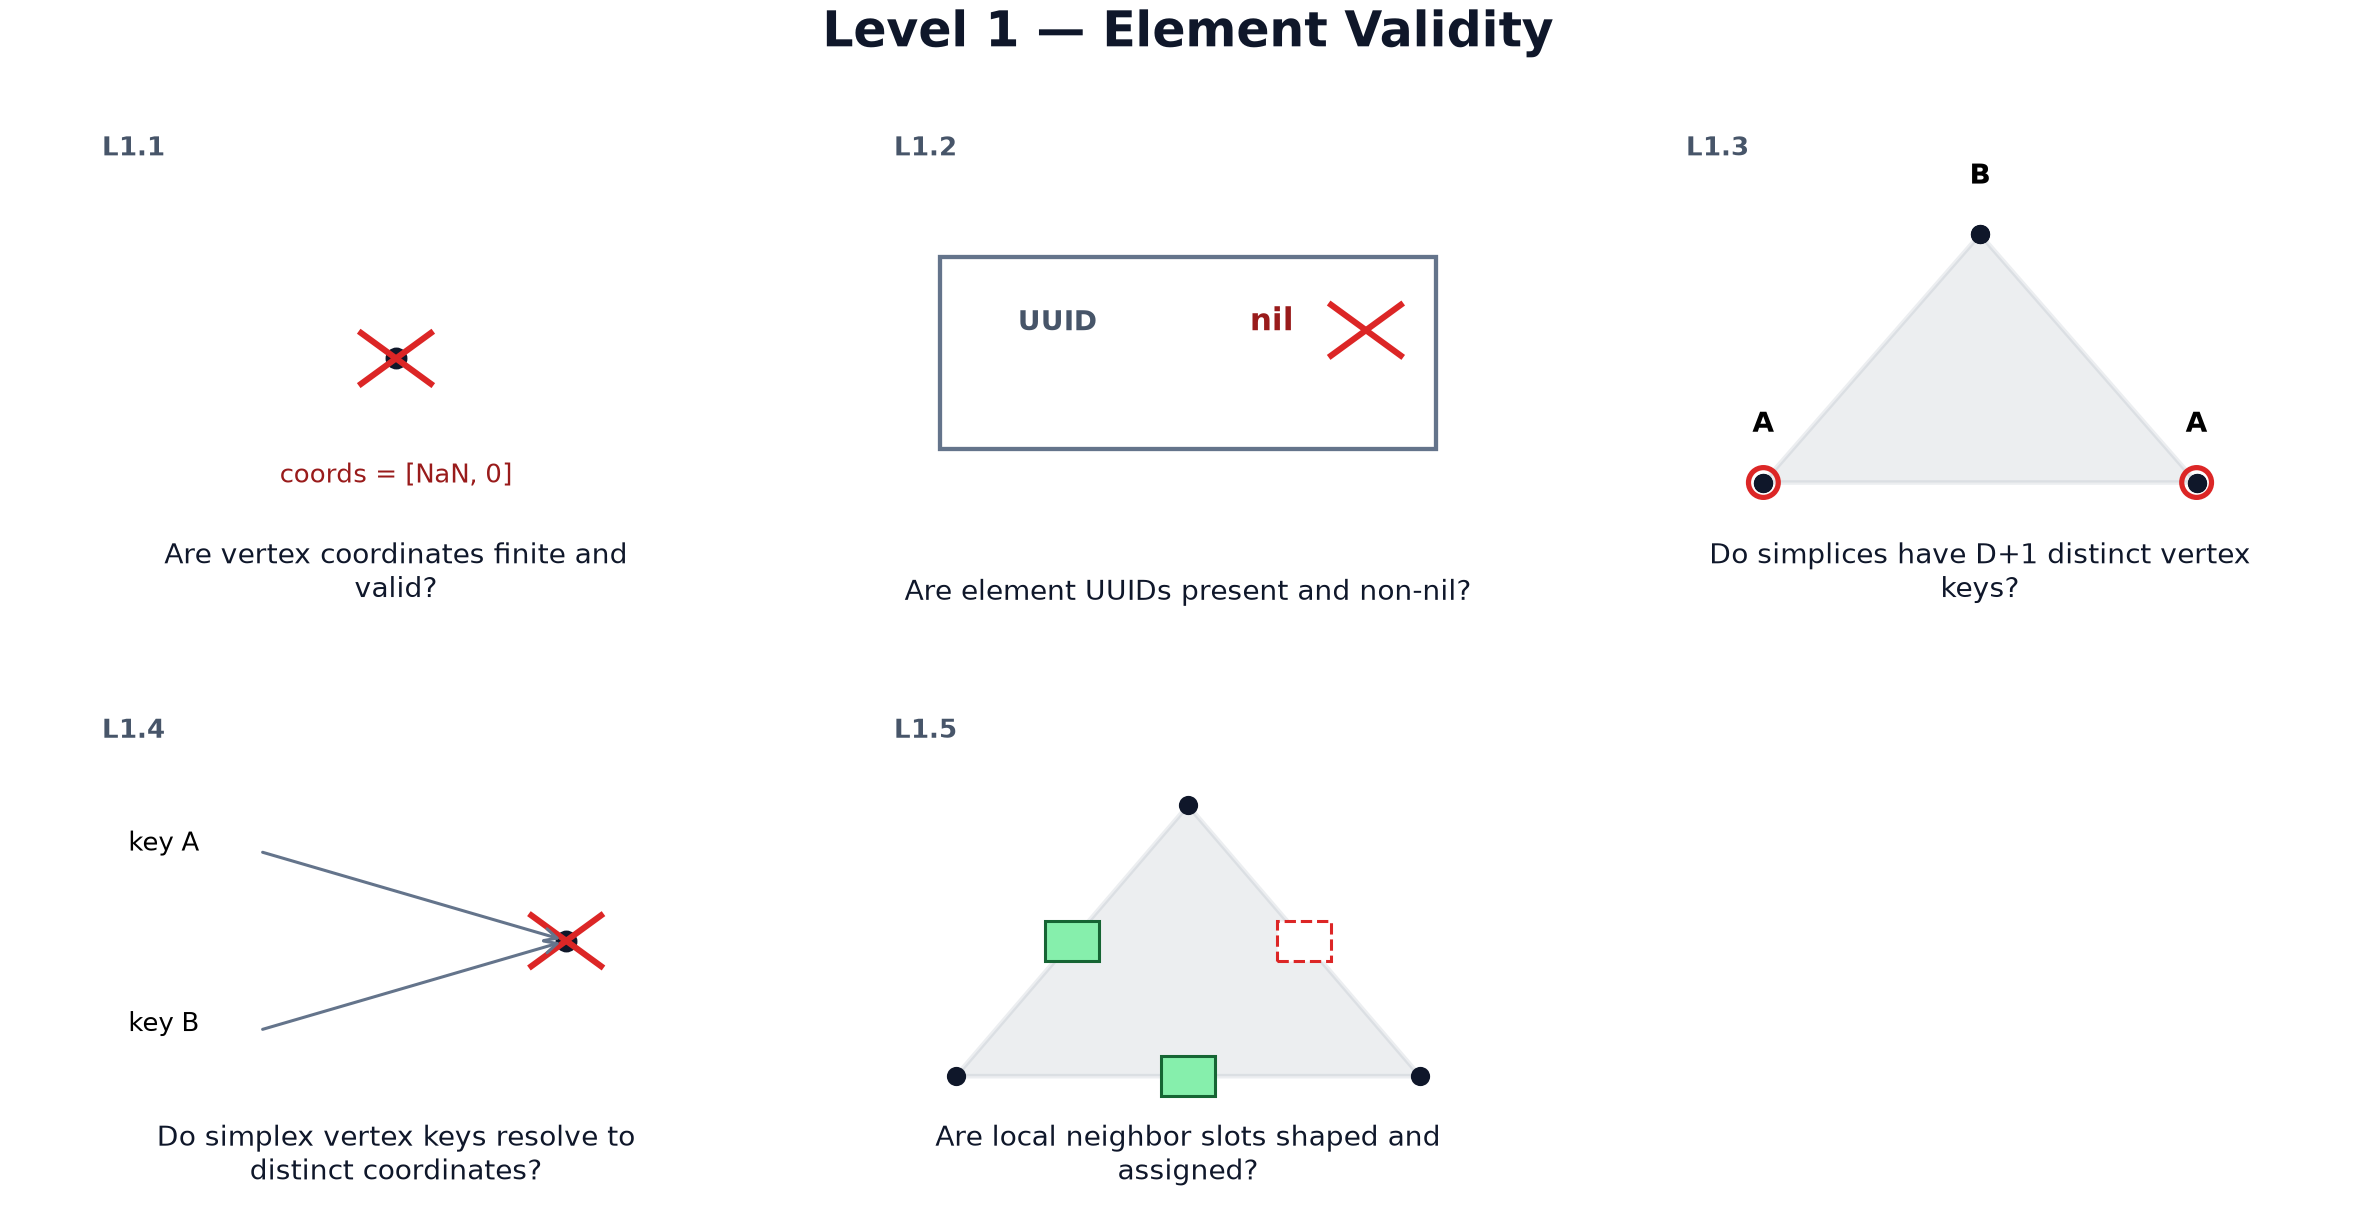
\includegraphics[width=0.88\linewidth]
  {../docs/assets/validation/validation_level_1_element_validity.png}
  \caption{\AuthorTodo{Describe the Level 1 validation witness figure.}}
  \label{fig:validation-level-1}
  \Description{Author TODO accessible description of the Level 1 validation
  witness figure.}
\end{figure}

\begin{figure}[p]
  \centering
  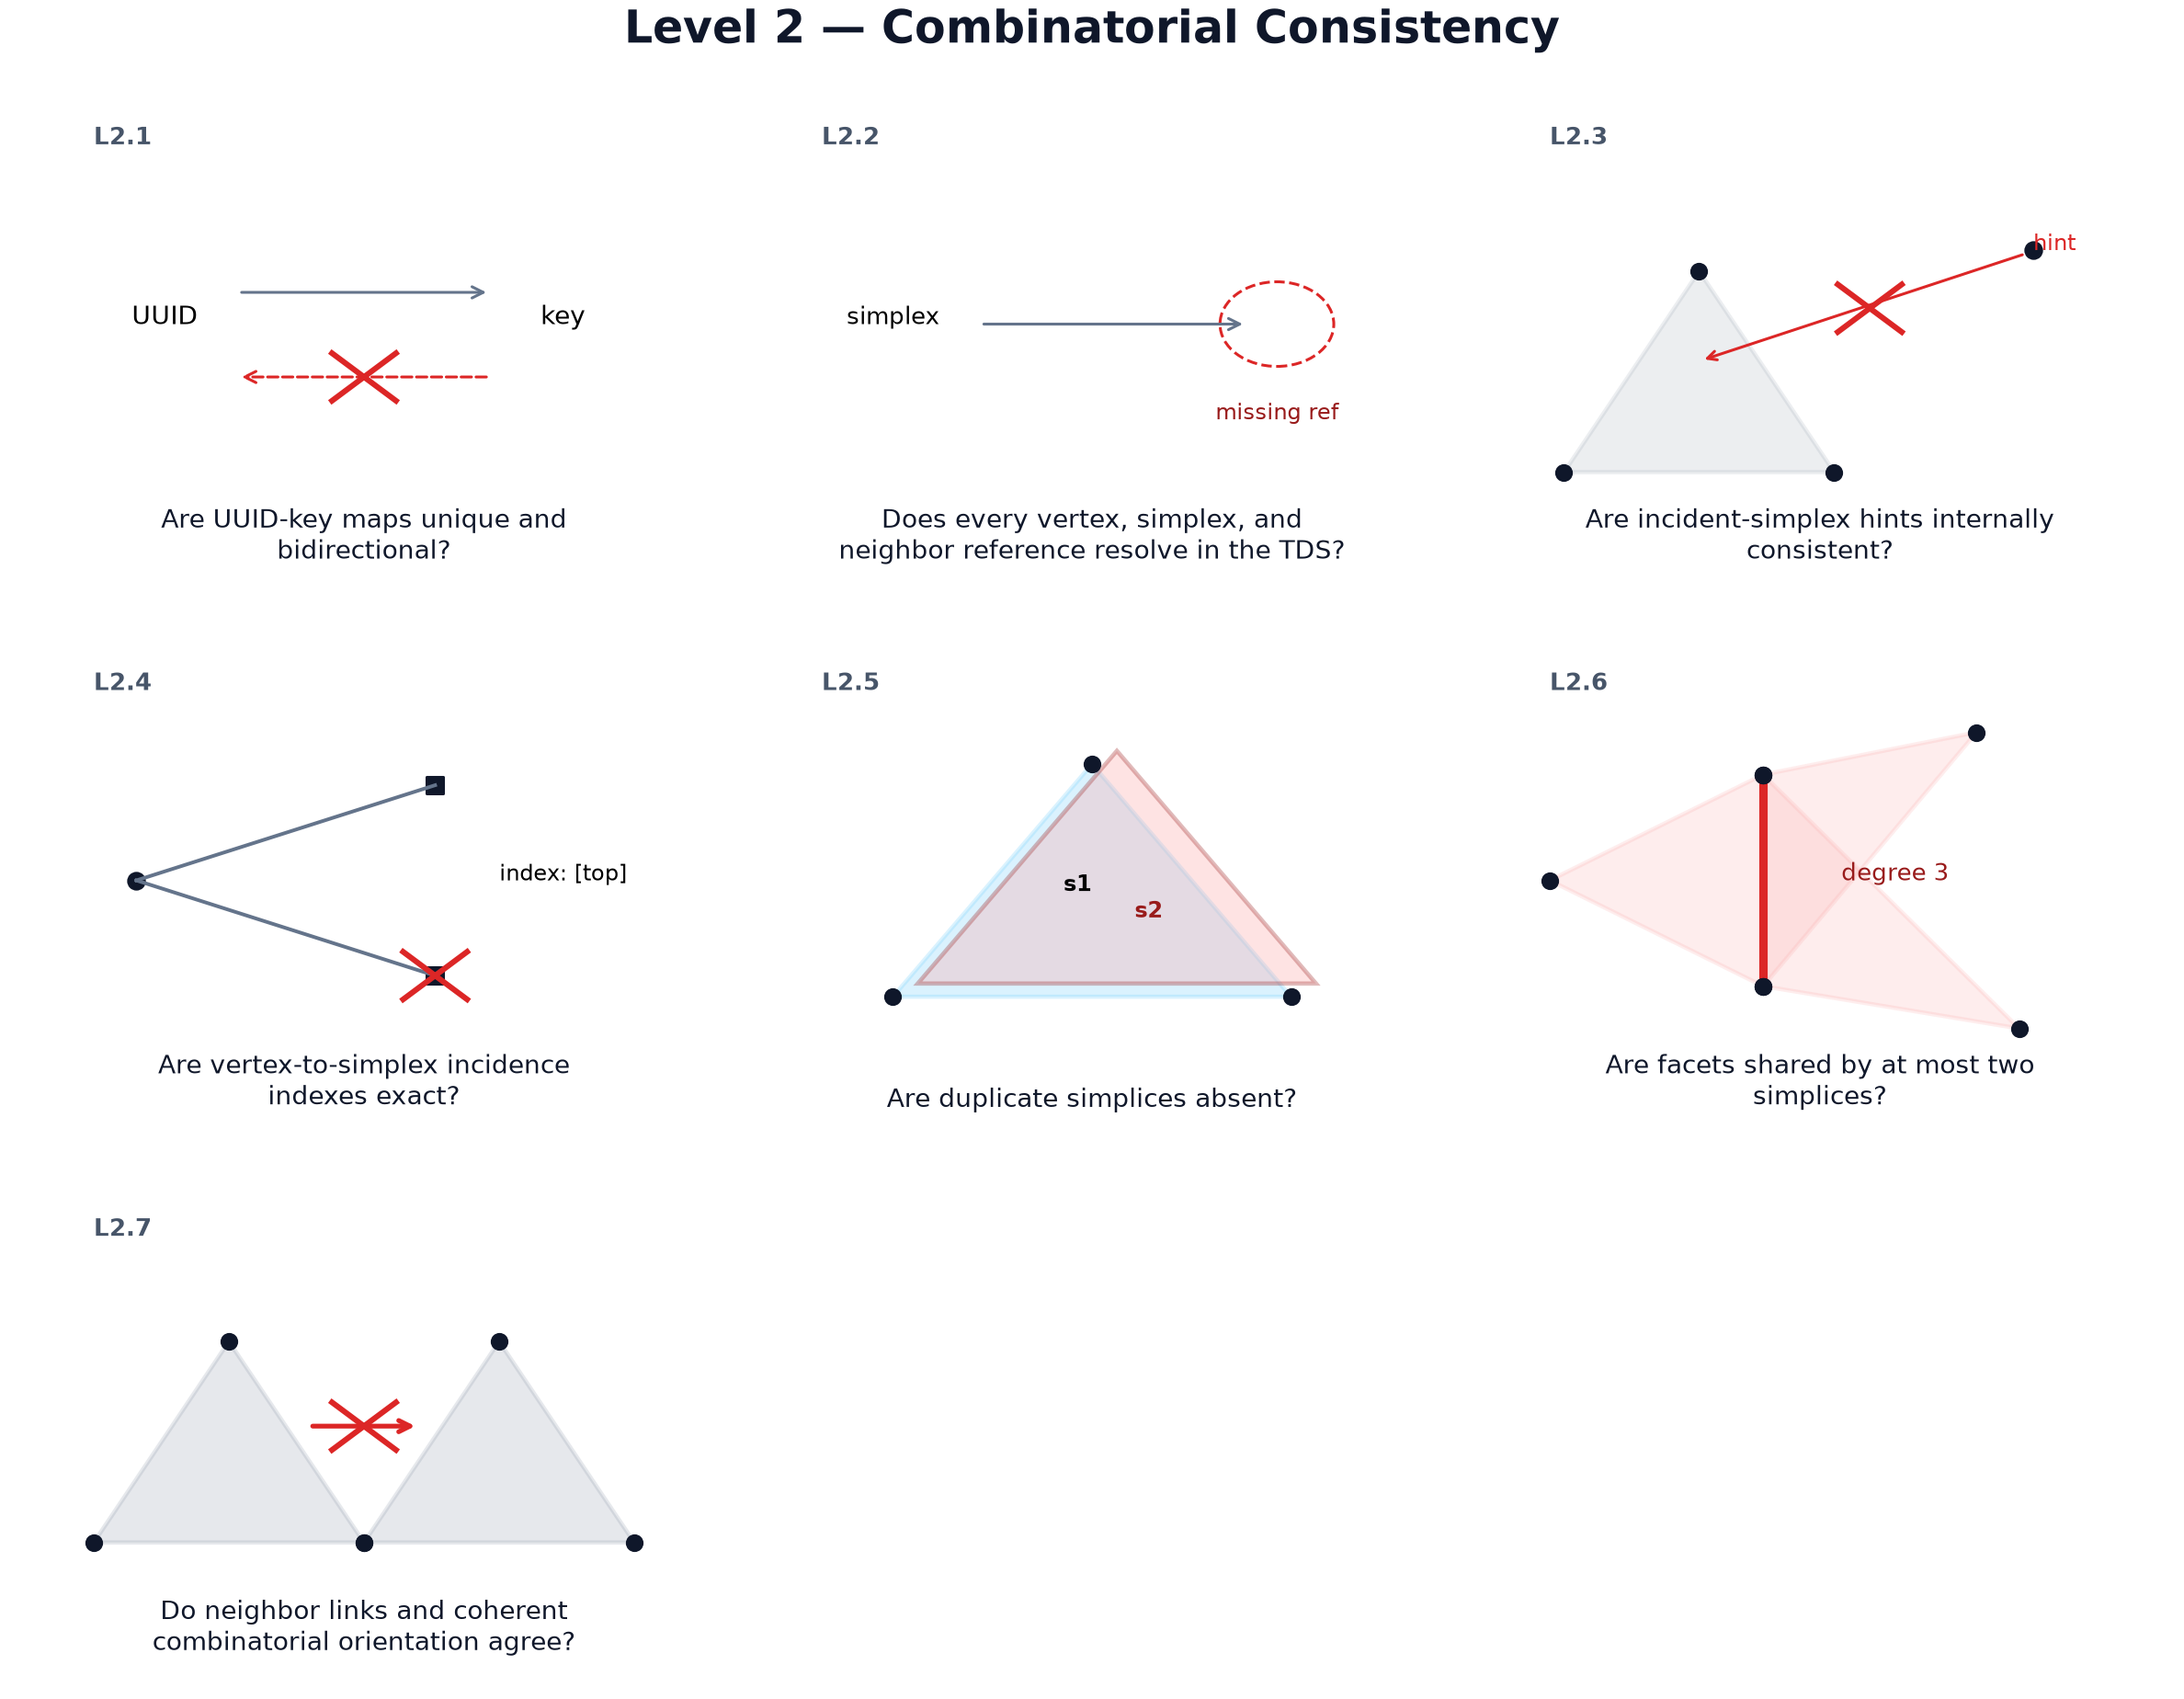
\includegraphics[width=0.88\linewidth]
  {../docs/assets/validation/validation_level_2_combinatorial_consistency.png}
  \caption{\AuthorTodo{Describe the Level 2 validation witness figure.}}
  \label{fig:validation-level-2}
  \Description{Author TODO accessible description of the Level 2 validation
  witness figure.}
\end{figure}

\begin{figure}[p]
  \centering
  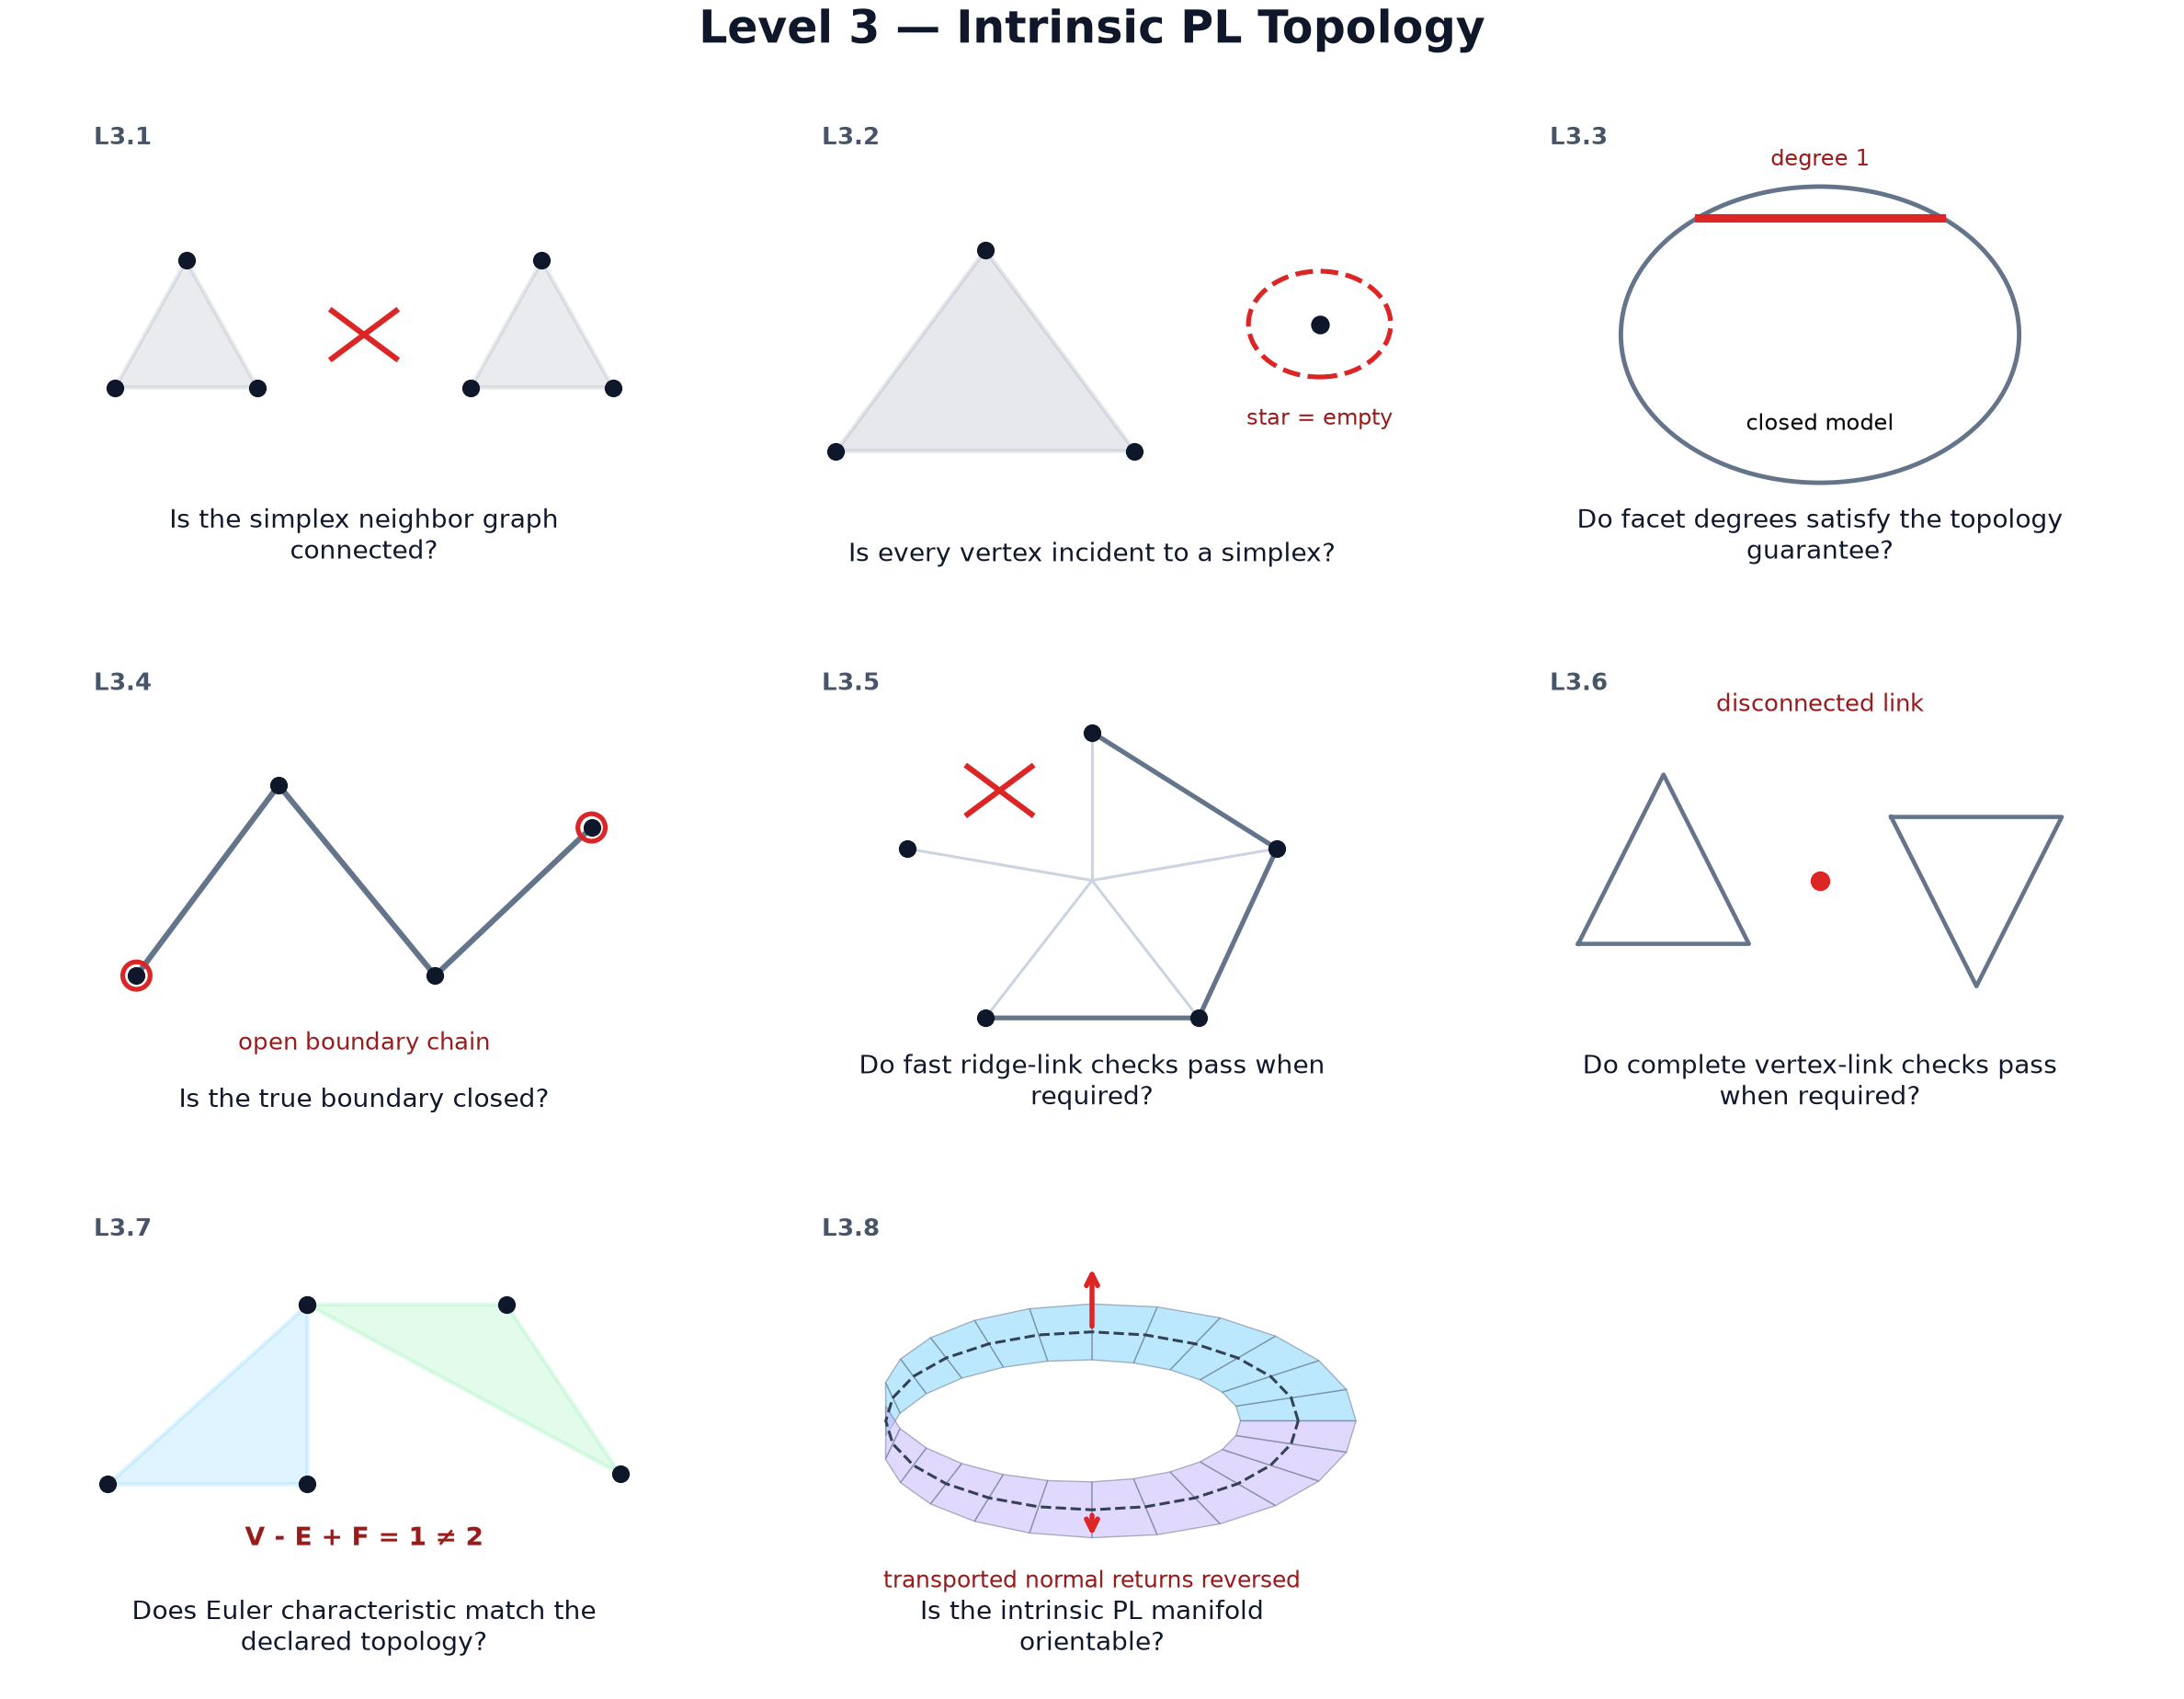
\includegraphics[width=0.88\linewidth]
  {../docs/assets/validation/validation_level_3_intrinsic_pl_topology.png}
  \caption{\AuthorTodo{Describe the Level 3 validation witness figure.}}
  \label{fig:validation-level-3}
  \Description{Author TODO accessible description of the Level 3 validation
  witness figure.}
\end{figure}

\begin{figure}[p]
  \centering
  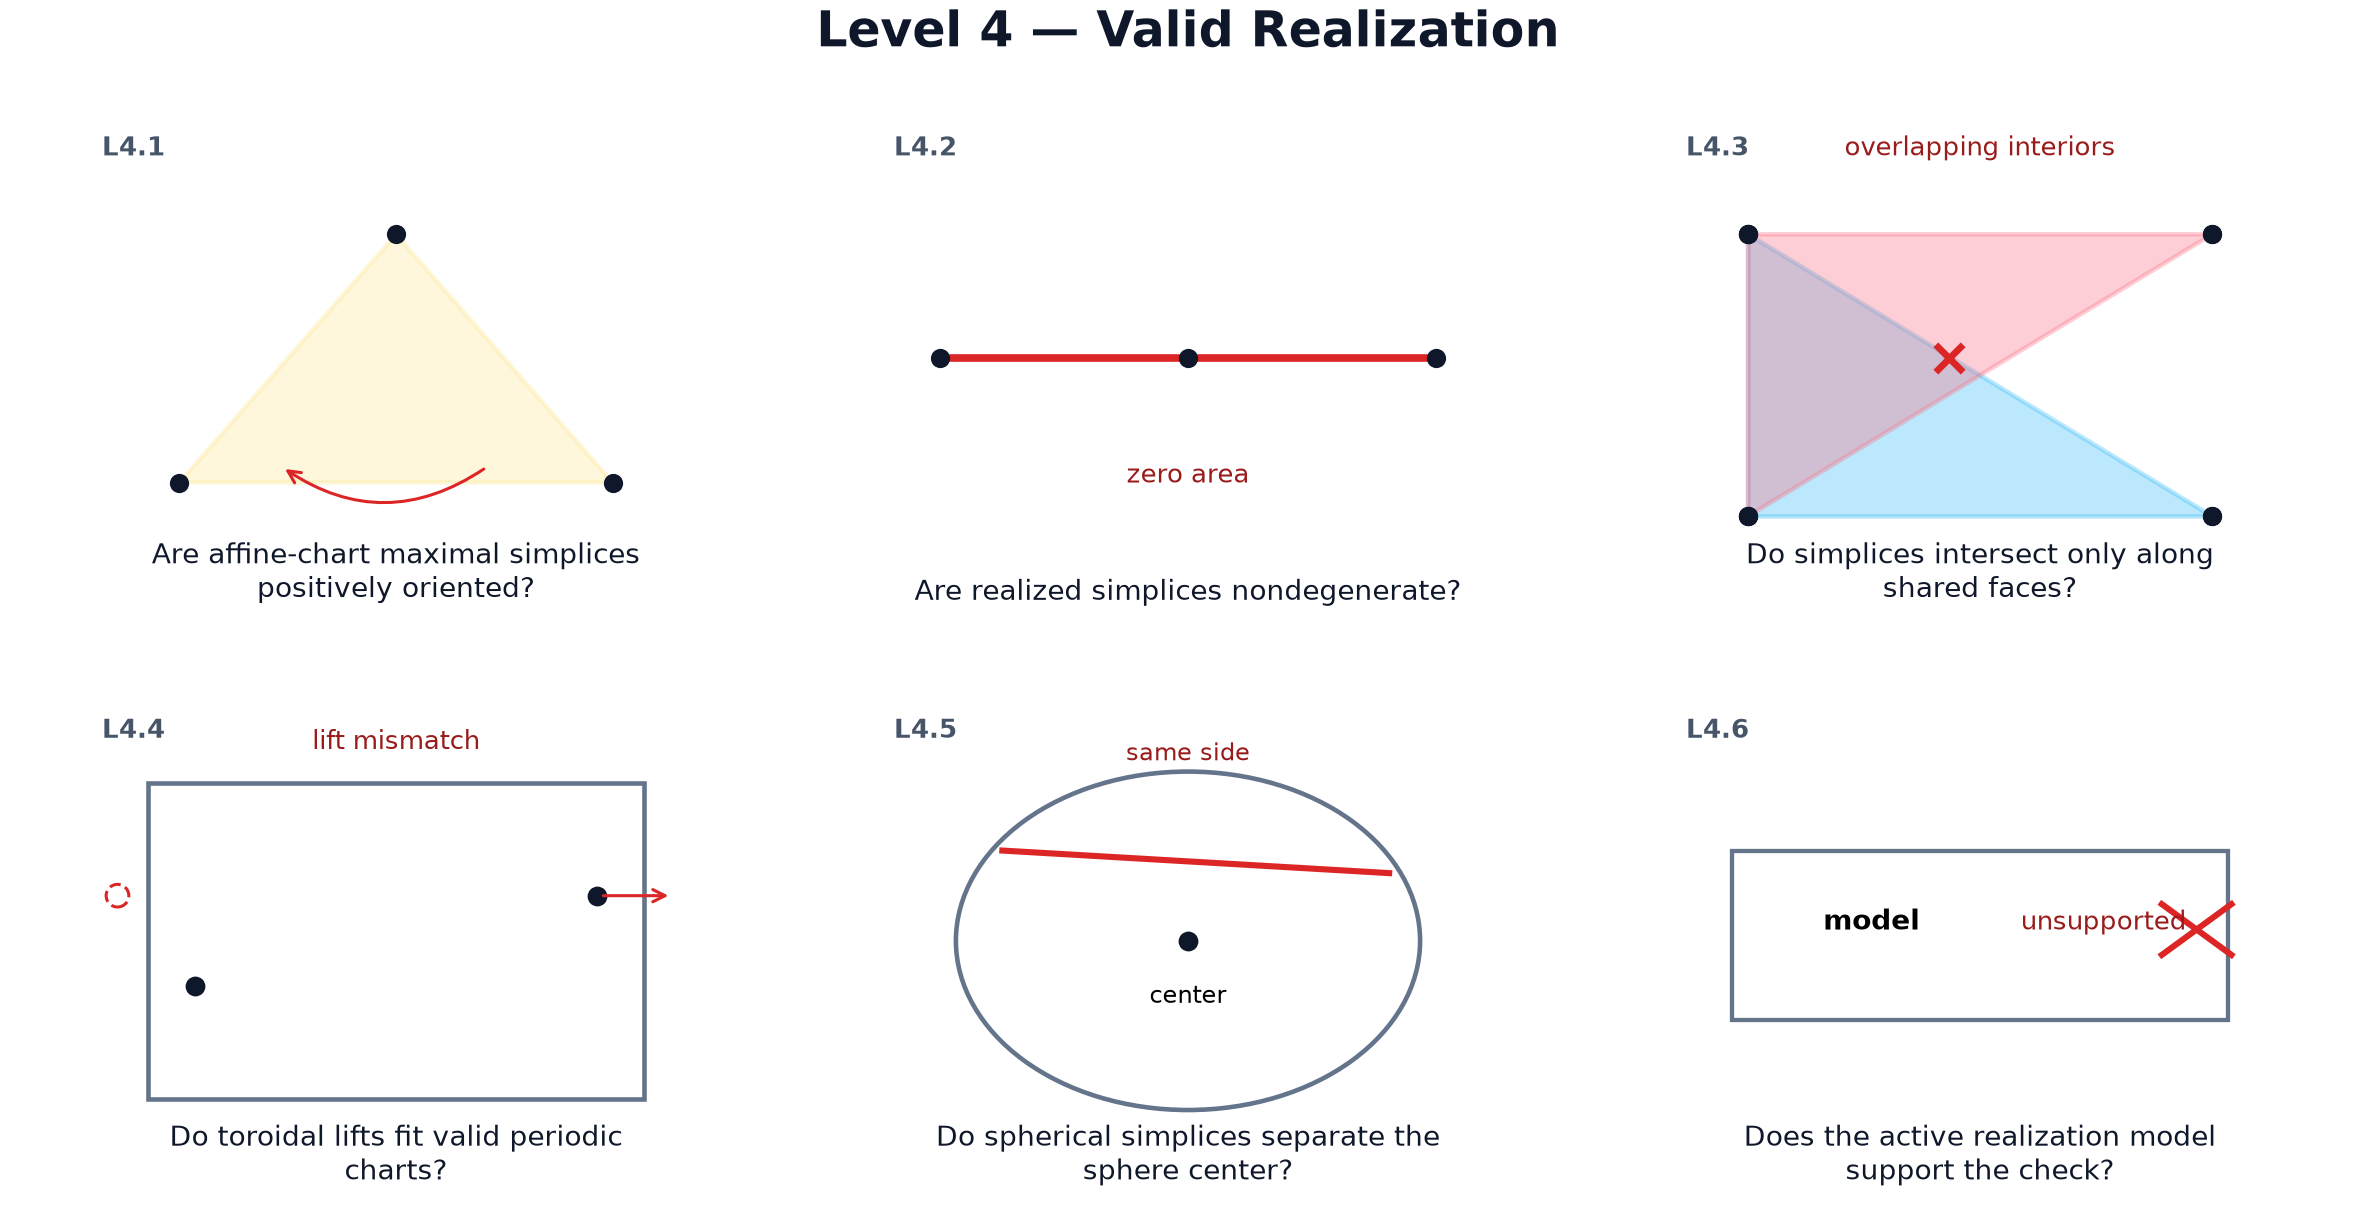
\includegraphics[width=0.88\linewidth]
  {../docs/assets/validation/validation_level_4_valid_realization.png}
  \caption{\AuthorTodo{Describe the Level 4 validation witness figure.}}
  \label{fig:validation-level-4}
  \Description{Author TODO accessible description of the Level 4 validation
  witness figure.}
\end{figure}

\clearpage
\begin{figure}[htbp]
  \centering
  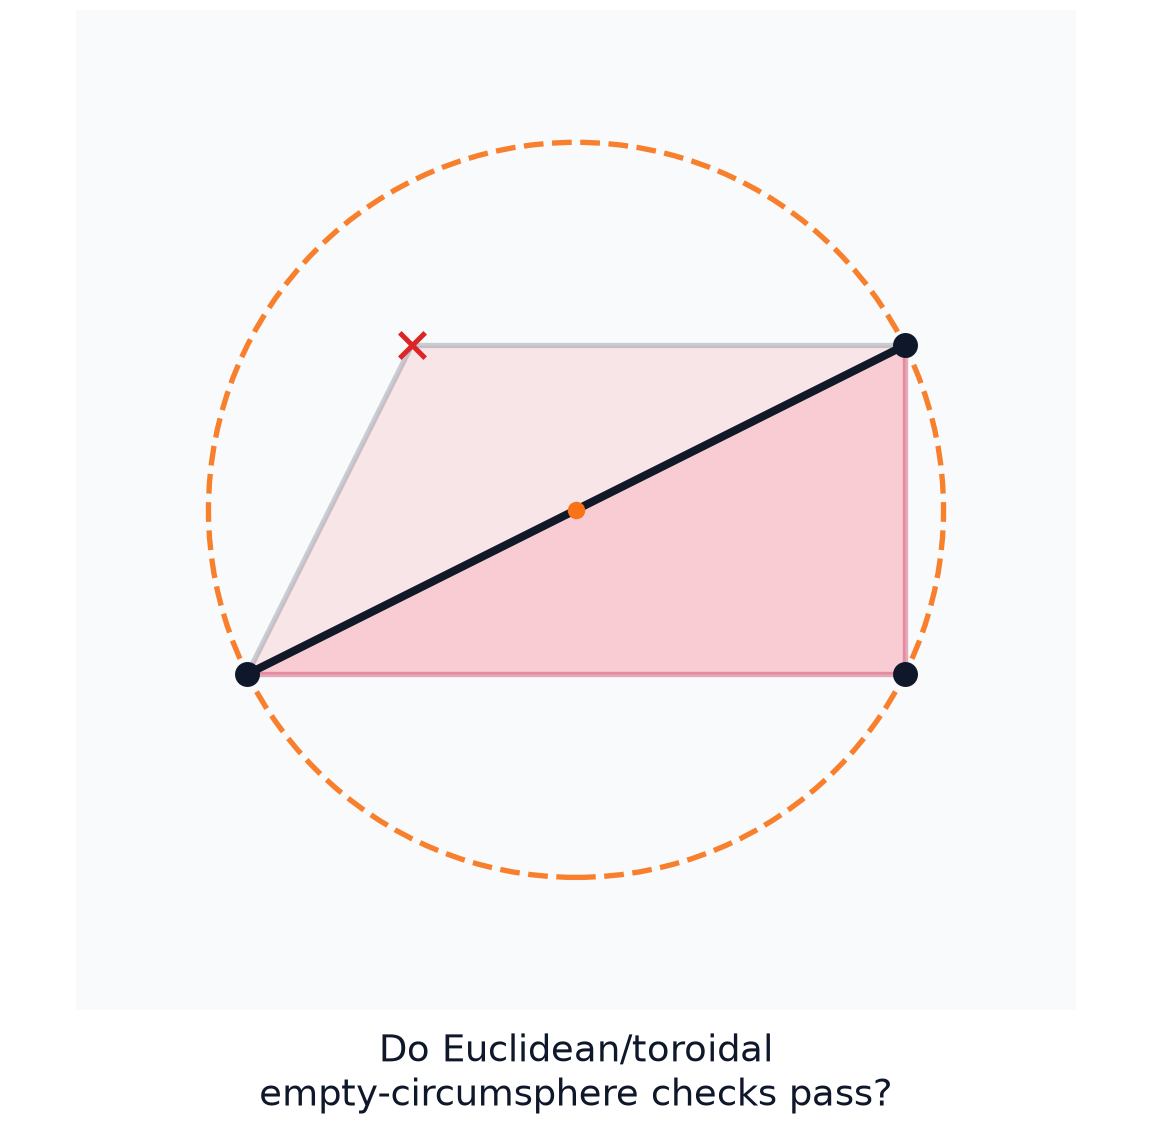
\includegraphics[width=0.52\linewidth]
  {../docs/assets/validation/validation_level_5_geometric_predicates.png}
  \caption{\AuthorTodo{Describe the Level 5 validation witness figure.}}
  \label{fig:validation-level-5}
  \Description{Author TODO accessible description of the Level 5 validation
  witness figure.}
\end{figure}

\begin{itemize}
  \item \AuthorTodo{Explain how the validation notebook generates paper
    figures.}
  \item \AuthorTodo{Describe representative diagnostics without duplicating API
    documentation.}
  \item \AuthorTodo{Connect figure generation to the reproducibility story.}
\end{itemize}

\section{Related Work}

\begin{itemize}
  \item \AuthorTodo{Place PL topology references and Pachner/Lickorish
    results.}
  \item \AuthorTodo{Place Euclidean robust-predicate and Delaunay references.}
  \item \AuthorTodo{Place spherical Delaunay and Riemannian-manifold
    references.}
  \item \AuthorTodo{Clarify which claims are architectural observations rather
    than literature claims.}
\end{itemize}

\section{Discussion and Future Work}

\begin{itemize}
  \item \AuthorTodo{Discuss extensibility to additional realization models and
    predicate families.}
  \item \AuthorTodo{Discuss limitations of the current implementation.}
  \item \AuthorTodo{Identify open validation and benchmarking questions.}
\end{itemize}

\section{Conclusion}

\begin{itemize}
  \item \AuthorTodo{Write the conclusion in your own words.}
\end{itemize}

\begin{acks}
  The author thanks Steven Carlip for discussions and guidance over
  the years on Causal Dynamical Triangulation, which motivated this work,
  and for encouragement and questions on this library, which
  motivated this paper.
\end{acks}

% Keep the reference list available in outline drafts so citation keys remain
% build-tested even before their final in-text placement is written
% by the author.
\nocite{*}
\bibliographystyle{ACM-Reference-Format}
\bibliography{validation}

\end{document}
